\documentclass[crop,tikz]{standalone}
\usepackage[english]{babel}
\usepackage{amsmath}
\usepackage[T1]{fontenc}
\usepackage[default]{droidsans}
\usepackage[LGRgreek]{mathastext}
\usetikzlibrary{decorations.text}
\usetikzlibrary{fadings}
\providecommand{\bsup}[1]{\mathbf{#1}}
\begin{document}
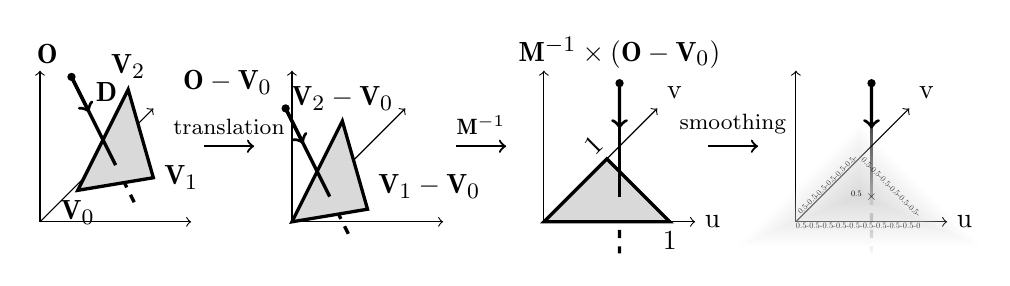
\begin{tikzpicture}[scale=1.6]

  % First coordinate system
  \draw[->] (0,0) -- (1.2,0);
  \draw[->] (0,0) -- (0,1.2);
  \draw[->] (0,0) -- (0.9,0.9);
  \begin{scope}[shift={(.3,.25)}]
    \begin{pgfinterruptboundingbox}
      \coordinate (O) at (-.05,0.9);
      \coordinate (inter) at (0.3,0.2);
      \path (O) -- (inter) coordinate[pos=1.5] (E);
    \end{pgfinterruptboundingbox}
    \draw[very thick, dashed] (inter) -- (E);
    \draw[very thick, fill=gray!30] (0.0,0.0) node[below, inner sep=3pt] {$\bsup{V}_0$} -- (0.6,0.1) node[right] {$\bsup{V}_1$} -- (0.4,0.8) node[above] {$\bsup{V}_2$} -- cycle;
    \draw[very thick] (O) node[inner sep=0pt, outer sep=0pt, minimum size=3pt, circle, fill, label=above left:{$\bsup{O}$}] {} -- (inter) coordinate[pos=0.4] (D);
    \draw[very thick, ->] (O) -- (D) node[above right,xshift=-1.5pt,] {$\bsup{D}$};
  \end{scope}

  % Arrow to second
  \draw[->, thick] (1.3,0.6) -- (1.7,0.6) node[midway, above, inner sep=4pt,font=\footnotesize] {translation};

  % Second coordinate system
  \begin{scope}[shift={(2,0)}]
    \draw[->] (0,0) -- (1.2,0);
    \draw[->] (0,0) -- (0,1.2);
    \draw[->] (0,0) -- (0.9,0.9);
    \begin{pgfinterruptboundingbox}
      \coordinate (O) at (-.05,0.9);
      \coordinate (inter) at (0.3,0.2);
      \path (O) -- (inter) coordinate[pos=1.5] (E);
    \end{pgfinterruptboundingbox}
    \draw[very thick, dashed] (inter) -- (E);
    \draw[very thick, fill=gray!30] (0.0,0.0) node[below, inner sep=3pt] {} -- (0.6,0.1) node[above right] {$\bsup{V}_1-\bsup{V}_0$} -- (0.4,0.8) node[above] {$\bsup{V}_2-\bsup{V}_0$} -- cycle;
    \draw[very thick] (O) node[inner sep=0pt, outer sep=0pt, minimum size=3pt, circle, fill, label=above left:{$\bsup{O}-\bsup{V}_0$}] {} -- (inter) coordinate[pos=0.4] (D);
    \draw[very thick, ->] (O) -- (D);
  \end{scope}

  % Arrow to third
  \draw[->, thick] (3.3,0.6) -- (3.7,0.6) node[sloped, midway, above,  inner sep=4pt, font=\footnotesize] {$\bsup{M}^{-1}$};

  % Third coordinate system
  \begin{scope}[shift={(4,0)}]
    \draw[->] (0,0) -- (1.2,0) node[right] {$u$};
    \draw[->] (0,0) -- (0,1.2);
    \draw[->] (0,0) -- (0.9,0.9) node[above right] {$v$};
    \begin{pgfinterruptboundingbox}
      \coordinate (O) at (.6,1.1);
      \coordinate (inter) at (0.6,0.2);
      \path (O) -- (inter) coordinate[pos=1.5] (E);
    \end{pgfinterruptboundingbox}
    \draw[very thick, dashed] (inter) -- (E);
    \draw[very thick, fill=gray!30] (0,0) -- (1,0) node[below, inner sep=3pt] {1} -- (.5,.5) node[above, rotate=45, inner sep=3pt] {1} -- cycle;
    \draw[very thick] (O) node[inner sep=0pt, outer sep=0pt, minimum size=3pt, circle, fill, label=above:{$\bsup{M}^{-1}\times\left(\bsup{O}-\bsup{V}_0\right)$}] {} -- (inter) coordinate[pos=0.4] (D);
    \draw[very thick, ->] (O) -- (D);
  \end{scope}

  % Arrow to fourth
  \draw[->, thick] (5.3,0.6) -- (5.7,0.6) node[sloped, midway, above,  inner sep=4pt,font=\footnotesize] {smoothing};

  \begin{pgfinterruptboundingbox}
    % Removed the unused `fade out` fading definition
    \tikzfading[name=fadeafter,
      bottom color=transparent!100,
      middle color=transparent!100,
    top color=transparent!50]
    \tikzfading[name=fadebefore,
      bottom color=transparent!75,
    top color=transparent!0]
  \end{pgfinterruptboundingbox}

  % Fourth coordinate system
  \begin{scope}[shift={(6,0)}]
    \draw[->] (0,0) -- (1.2,0) node[right] {$u$};
    \draw[->] (0,0) -- (0,1.2);
    \draw[->] (0,0) -- (0.9,0.9) node[above right] {$v$};
    \begin{pgfinterruptboundingbox}
      \coordinate (O) at (.6,1.1);
      \coordinate (inter) at (0.6,0.2);
      \path (O) -- (inter) coordinate[pos=1.5] (E);
      \draw[very thick, dashed, path fading=fadeafter] (inter) -- (E);
    \end{pgfinterruptboundingbox}

    % --- Replaced circular fading with exact incenter-scaled distance fading ---
    % Incenter for triangle (0,0), (1,0), (0.5,0.5) is (0.5, 0.20710678)
    \def\incenterX{0.5}
    \def\incenterY{0.20710678}
    \foreach \i in {1,2,...,40} {
      % Scale from 2.0 (outside) down to 0.0 (center)
      \pgfmathsetmacro{\s}{2.0 - \i*0.05}

      % Calculate required layer opacity to ensure linear accumulation (0.5 at boundary)
      \pgfmathsetmacro{\alpha}{\i == 40 ? 1.0 : 0.025 / (1.0 - (\i-1)*0.025)}

      % Scale each vertex relative to the incenter
      \pgfmathsetmacro{\vAx}{\incenterX + \s*(0.0 - \incenterX)}
      \pgfmathsetmacro{\vAy}{\incenterY + \s*(0.0 - \incenterY)}
      \pgfmathsetmacro{\vBx}{\incenterX + \s*(1.0 - \incenterX)}
      \pgfmathsetmacro{\vBy}{\incenterY + \s*(0.0 - \incenterY)}
      \pgfmathsetmacro{\vCx}{\incenterX + \s*(0.5 - \incenterX)}
      \pgfmathsetmacro{\vCy}{\incenterY + \s*(0.5 - \incenterY)}

      \fill[gray!30, opacity=\alpha] (\vAx,\vAy) -- (\vBx,\vBy) -- (\vCx,\vCy) -- cycle;
    }
    % ---------------------------------------------------------------------------

    \draw[decorate, decoration={text effects along path,
        text={0.5-},
        raise=-2.5pt,
        post length=1pt,
        text effects/.cd,
        repeat text,
        character count=\m, character total=\n,
    characters={text along path, scale=0.3, opacity=0.75}}]
    (0,0) -- (1,0);
    \draw[decorate, decoration={text effects along path,
        text={0.5-},
        raise=+0pt,
        pre length=1pt,
        post length=2pt,
        text effects/.cd,
        repeat text,
        character count=\m, character total=\n,
    characters={text along path, scale=0.3, opacity=0.75}}]
    (.5,.5) -- (1,0);
    \draw[decorate, decoration={text effects along path,
        text={0.5-},
        raise=+.5pt,
        pre length=3pt,
        text effects/.cd,
        repeat text,
        character count=\m, character total=\n,
    characters={text along path, scale=0.3, opacity=0.75}}]
    (0,0) -- (.5,.5) ;
    \node[opacity=0.75, scale=0.5, label={[right, xshift=-2.5pt, yshift=-2.4pt, anchor=east, scale=0.3]:0.5}] at (inter) {$\times$};
    \draw[very thick, path fading=fadebefore] (O) -- (inter) coordinate[pos=0.4] (D);
    \draw[very thick, ->] (O) node[inner sep=0pt, outer sep=0pt, minimum size=3pt, circle, fill] {} -- (D);
  \end{scope}

\end{tikzpicture}
\end{document}
